\documentclass{article}
\usepackage{graphicx}

\title{
    \textbf{pacman-racket} \\
    \textit{Developer Guide}\\
    A pragmatic implementation of Pacman in Racket
}

\author{
    Alessandro Zanzi,
    Filippo Piloni,\\
    Jeferson Morales Mariciano,
    Paolo Deidda
}

\date{
    USI \\
    Faculty of Informatics \\
    [\baselineskip]  2021/2022
}


\begin{document}
%%%%%%%%%%%%%%%%%%%%%%%
%%%%%%%%%%%%%%%%%%%%%%%
%%%%%%%%%%%%%%%%%%%%%%%
\begin{titlepage}
\maketitle  
\thispagestyle{empty}
\end{titlepage}
%%%%%%%%%%%%%%%%%%%%%%%
%%%%%%%%%%%%%%%%%%%%%%%
%%%%%%%%%%%%%%%%%%%%%%%
%%%%%%%%%%%%%%%%%%%%%%%
%%%%%%%%%%%%%%%%%%%%%%%
%%%%%%%%%%%%%%%%%%%%%%%
\tableofcontents
\clearpage
%%%%%%%%%%%%%%%%%%%%%%%
%%%%%%%%%%%%%%%%%%%%%%%
%%%%%%%%%%%%%%%%%%%%%%%
\section{Assumptions}
It is assumed that developers read also the user guide in order to achieve a better understanding of the game rules, interactions, program UI and general knowledge of the gameflow.

\section{Analysis}

\hspace{0.5cm}\textbf{Modularity}\\
 In order for the group to work in parallel on the project we created several files on which each of us worked simultaneously. These files were then interconnected with the built-in function of Racket "require" followed by the name of the file.

\begin{center}
 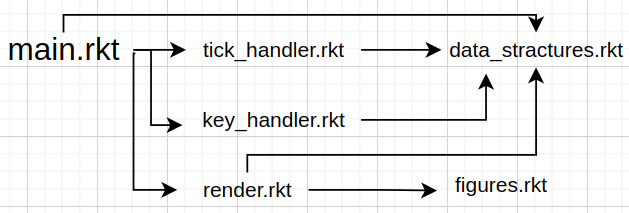
\includegraphics[width=12cm]{images/dependency_tree.png}
\end{center}
 
\textbf{Bottom-up approach}\\
We developed the code decomposing the functions needed in the simplest possible problems, we then conveyed them in higher grade functions. This allowed a design recipe with more tests making the debugging process easier.
 
\begin{center}
 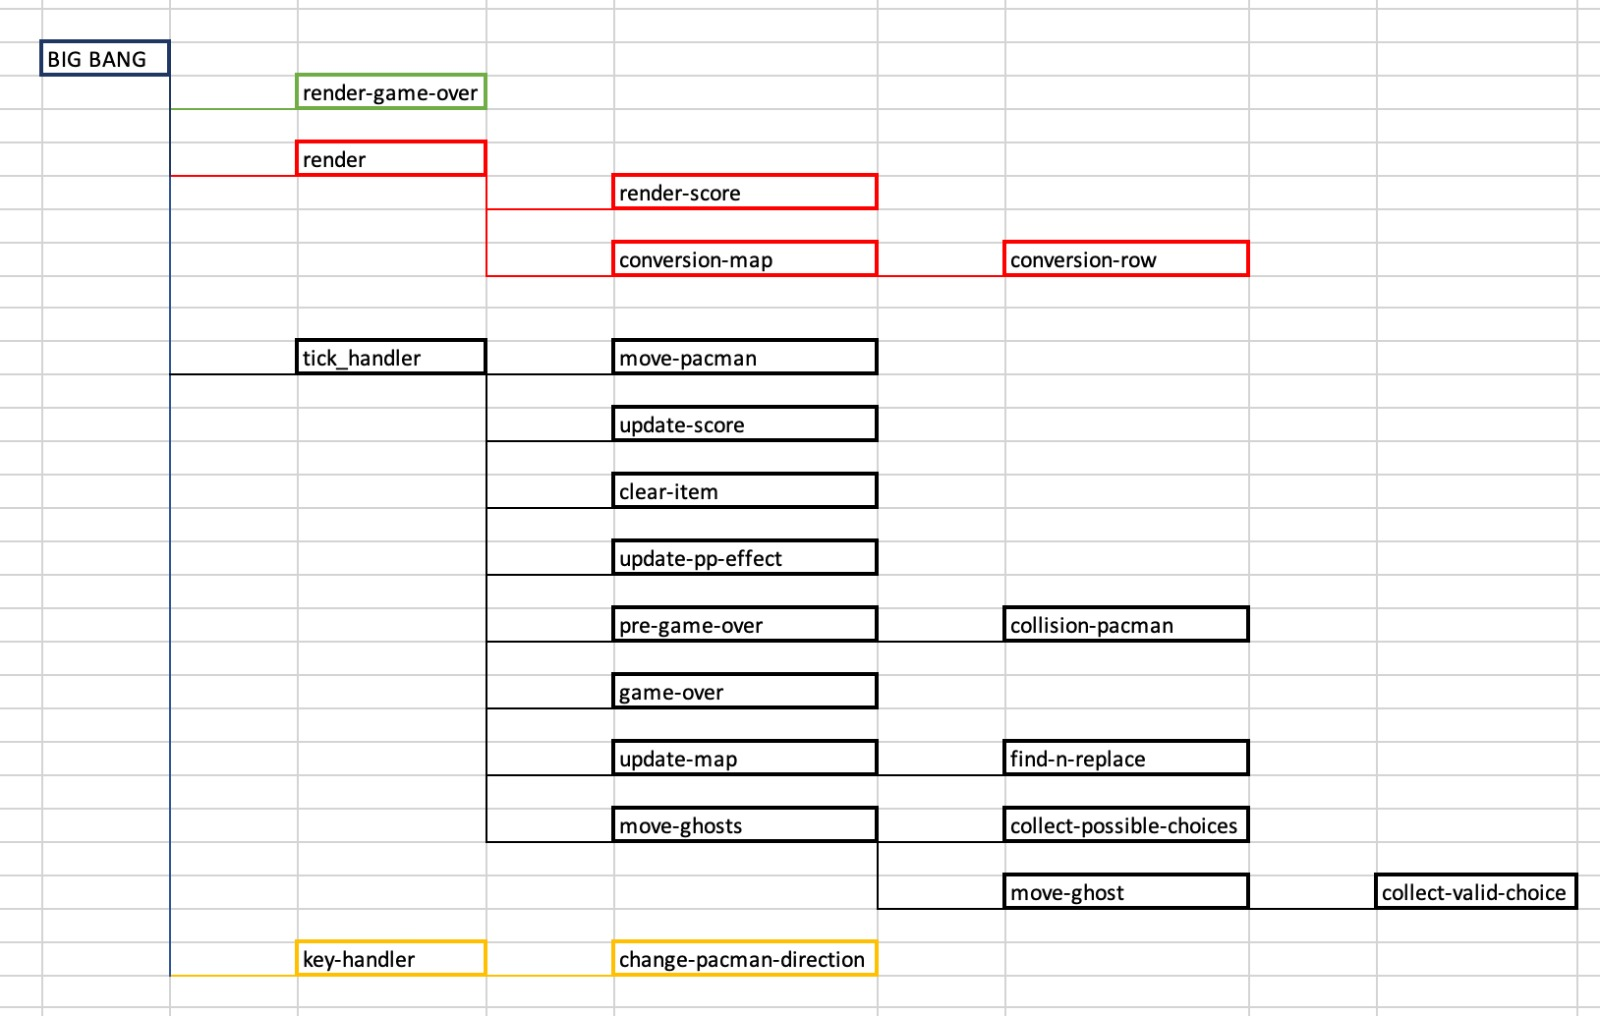
\includegraphics[width=12cm]{images/dependency_tree2.jpeg}
\end{center}
 
%%%%%%%%%%%%%%%%%%%%%%%
%%%%%%%%%%%%%%%%%%%%%%%
%%%%%%%%%%%%%%%%%%%%%%%
\section{Sofware design}
\subsection{Tools}
\hspace{0.5cm}\LaTeX \\
Used for the user and developer guide.\\
 
\textit{Flowchart}\\
Used to create the dependency and function trees, so each member of the group had a clear view of the whole project.

\subsection{Main Functions}
The main function of the program is the BIG-BANG function (avaible in main.rkt). It operates using four principal sub-functions which purpose is explain below:\\\\
- \textbf{render} : renders the map as a matrix of images. The function, given a list of lists of images it elaborates them, putting the images beside and above each other to create the map.\\
- \textbf{tick-handler} : Given an appstate, it split it in the various parts: at each movement from a character, first pacman then the ghosts, updates the map; updates powerpellet and score if needed and checks if the game ended by setting the quit status. Finally, he puts them all together in an appstate that will be evaluated by the render.\\
- \textbf{key-handler} : changes the direction value of pacman struct in the appstate according to the arrow key stroke. 
Stops the program is '\textit{q}' is pressed.\\
- \textbf{render-game-over} : Given an appstate, it returns an image when the game ends with the evaluation of the total point and the overlayed text with ``\textit{GAME OVER}'' or ``\textit{YOU WON}''.

%%%%%%%%%%%%%%%%%%%%%%%
%%%%%%%%%%%%%%%%%%%%%%%
%%%%%%%%%%%%%%%%%%%%%%%
\section{Software Development}

\subsection{Source Code}
The project is developed on the idea of creating a map of squares placed side by side that make up the game world. To run the game, we work on a "logic map" which is composed by strings of characters, that form lines, one above the other. This set of lines creates a vector that will be the game logic map. All the engine functions that we have developed in the source code operate on the lines of this vector in a recursive manner modifying and moving the various characters.To give life to the game we then have created a render function that takes each character of the logic map and associates the corresponding image.\\
 
\begin{center}
 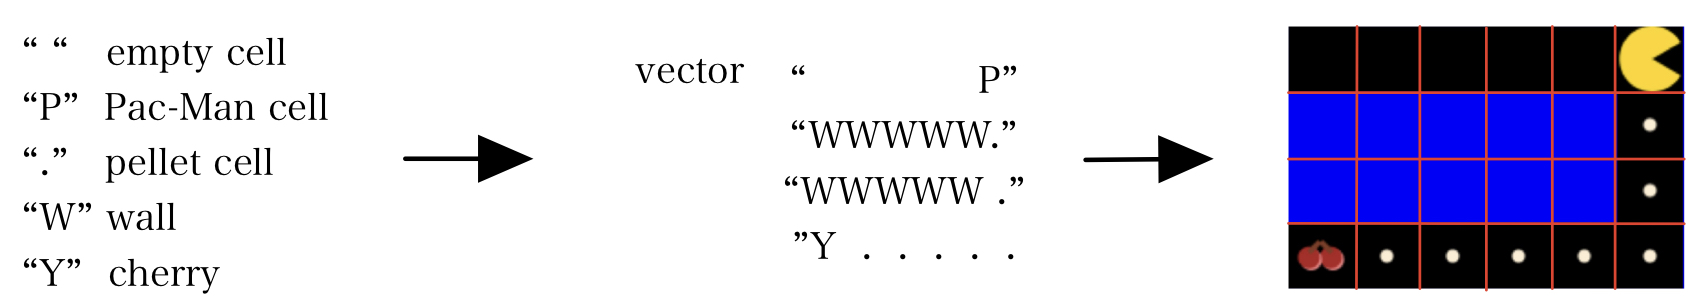
\includegraphics[width=12cm]{./images/vector.jpeg}
\end{center}

Characters such as Pac-Man and ghosts are defined by structures in the code. Pac-Man movement direction is defined by the key-events: arrow '\textit{up}', '\textit{down}', '\textit{left}', '\textit{right}'.
Instead, ghosts movement are defined randomly between the possible available near cells. When Pac-Man is one cell distant, ghosts start to follow it.
As an example for Pacman, the validity of its moves is verified by checking what is in the current and next cell and the event about to happen like collision with a ghost, a wall, a powerpellet, etc. Likewise, at runtime when there is a wall in the next box, the \textit{(move-pacman)} function returns pacman to the same position, if instead there is an invulnerable ghost the game over event will be triggered.
 
\subsection{Tools}
 
\hspace{0.5cm}\textit{Racket}\\
Programming language used to develop the game.
We specifically used the teach language: Advance Student.\\
 

\textit{DrRacket}\\
Used as Integrated development environment (IDE).\\
 
\textit{VCS Git}\\
Software that we used to track changes in the project set of files, in order to each of us to develop source code and share it in an easy and reliable way: low risk of data loss and archives with the previous versions ready to back up if needed.\\

\textit{Hosting GitHub}\\
The whole project is physically stored in a private repository located on GitHub's servers. This granted us to access the work at any time in any place as long as we had internet connection.

\subsection{Libraries}
\hspace{0.5cm}\textit{Universe}\\
Teachpack that implements and provides the functionality for creating interactive, graphical programs that consist of plain mathematical functions.

\textit{Image}\\
The image teachpack provides a number of basic image construction functions, along with combinators for building more complex images out of existing images.

%%%%%%%%%%%%%%%%%%%%%%%
%%%%%%%%%%%%%%%%%%%%%%%
%%%%%%%%%%%%%%%%%%%%%%%

\end{document}
